\section{Benchmark}
\label{eval}
To evaluate Yarn, it's performance will be analyzed first by itself, then it
is compared to the other Ruby webservers covered in Section~\ref{webservers}.
The measure of performance is how many requests the webserver can handle per
second. The tests were run on a Linux machine with four cores and 8GB RAM.

\subsection{Yarn Performance}
To get an idea of the performance of Yarn, it was measured how many requests
per second (req/sec) it could handle at different counts of worker processes.
Figure~\ref{optwork} plots Yarn performance.

\begin{figure}[htb]
  \centering
  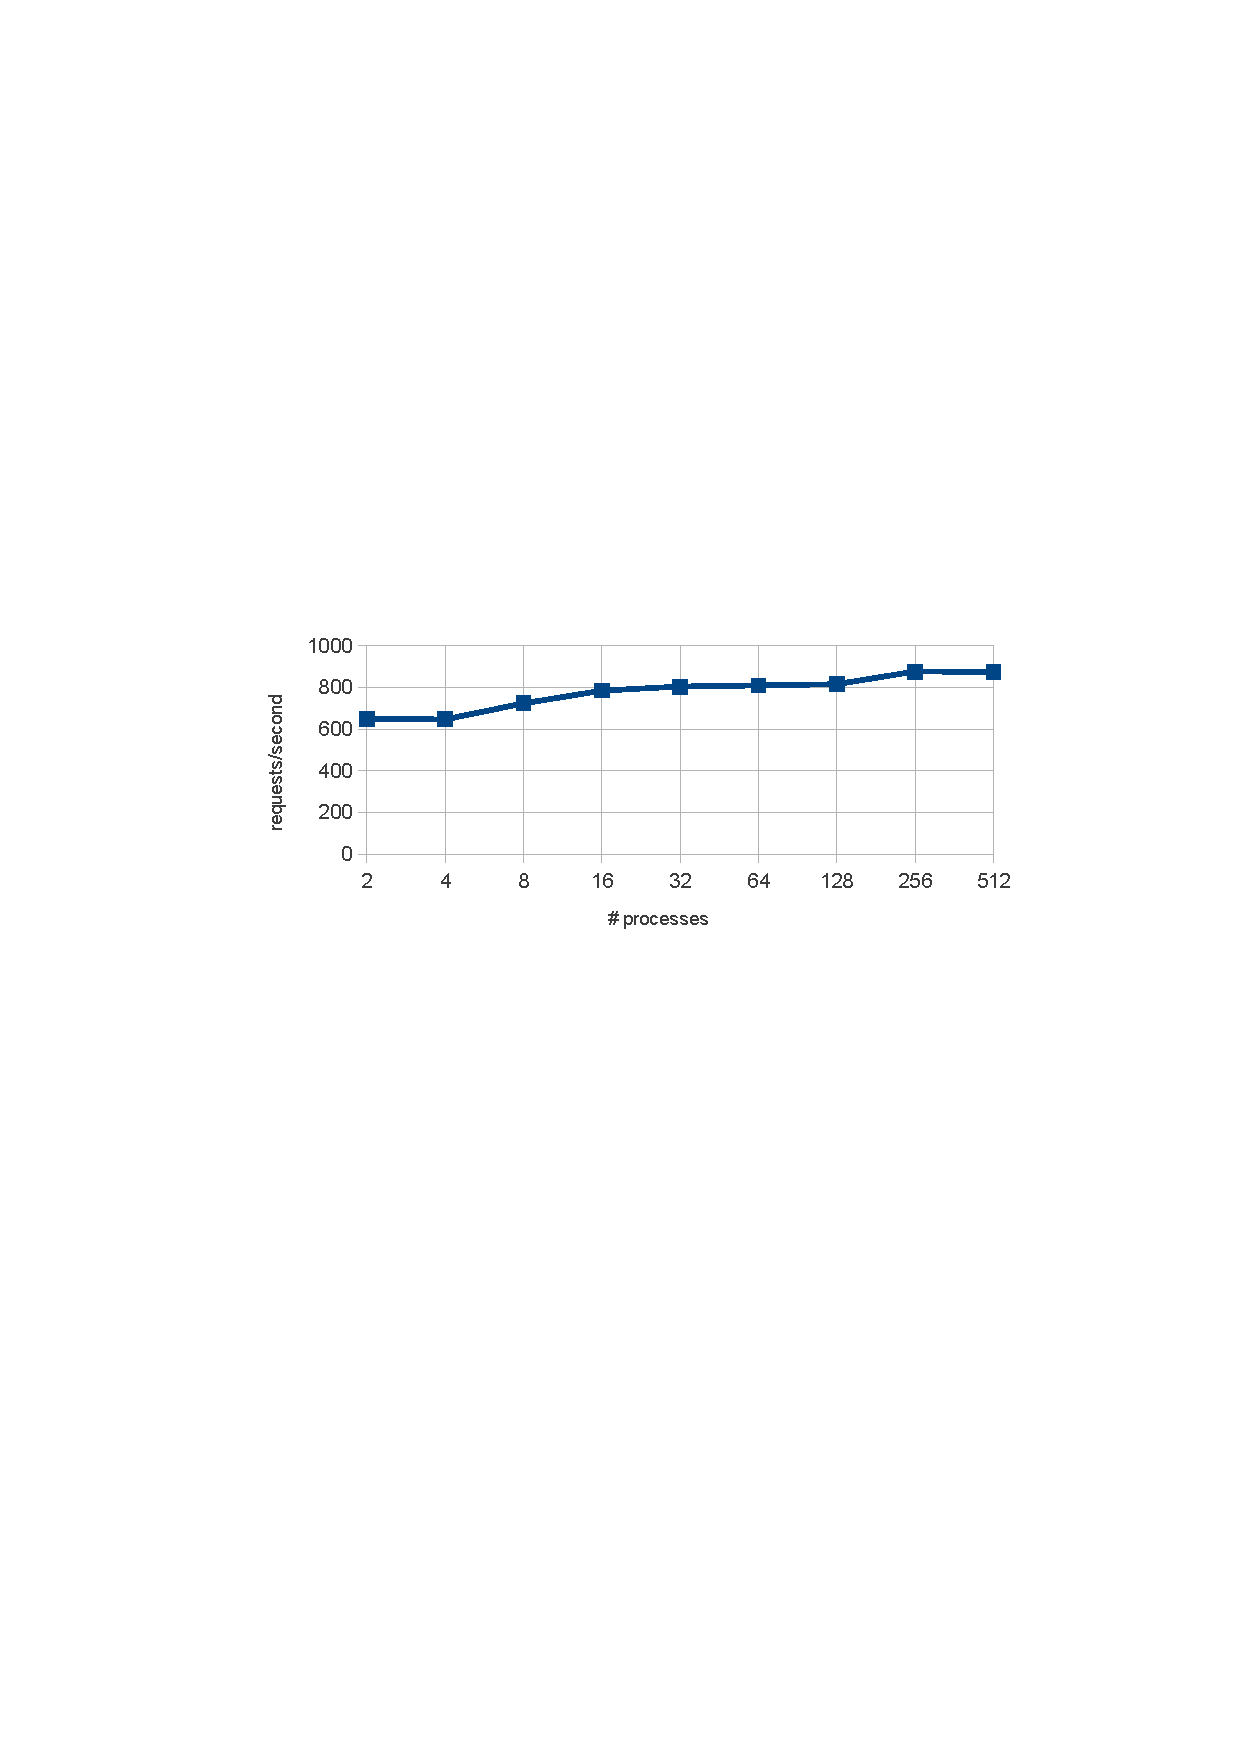
\includegraphics[width=1.0\textwidth]{results/optimal_workers_crop.pdf}
  \caption{Yarn req/sec}
  \label{optwork}
\end{figure}

Test runs above 512 processes bogged the computer down and were not included.
The best result was achieved with 256 worker processes with 875
req/sec, and on average Yarn performed 775 req/sec. The test consisted of
making 1000 requests, 20 at a time, to Yarn serving a simple Rack application.

\subsection{Yarn Vs. Other Ruby Webservers}

